\chapter{Algoritmos de linha de varredura}

\index{linha de varredura}

Muitos problemas geométricos podem ser resolvidos usando
algoritmos de \key{linha de varredura}.
A ideia em tais algoritmos é representar
uma instância do problema como um conjunto de eventos que correspondem
a pontos no plano.
Os eventos são processados em ordem crescente
de acordo com suas coordenadas x ou y.

Como exemplo, considere o seguinte problema:
Há uma empresa que tem $n$ funcionários,
e sabemos para cada funcionário seus horários de chegada e
saída em um determinado dia.
Nossa tarefa é calcular o número máximo de
funcionários que estavam no escritório ao mesmo tempo.

O problema pode ser resolvido modelando a situação
de forma que cada funcionário receba dois eventos que
correspondem aos seus horários de chegada e saída.
Após ordenar os eventos, nós os percorremos
e mantemos o controle do número de pessoas no escritório.
Por exemplo, a tabela
\begin{center}
\begin{tabular}{ccc}
pessoa & horário de chegada & horário de saída \\
\hline
João & 10 & 15 \\
Maria & 6 & 12 \\
Pedro & 14 & 16 \\
Lisa & 5 & 13 \\
\end{tabular}
\end{center}
corresponde aos seguintes eventos:
\begin{center}
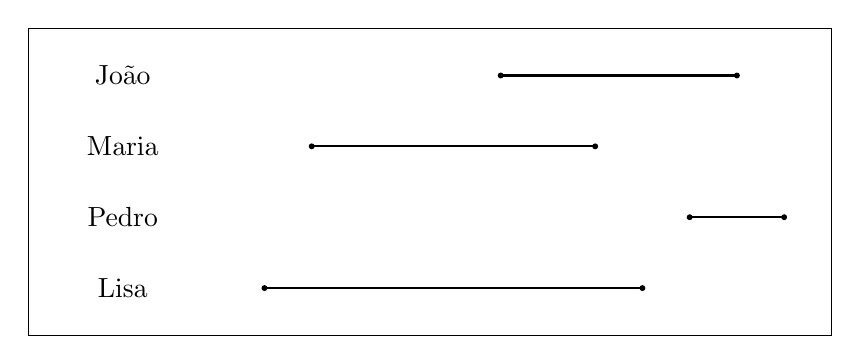
\begin{tikzpicture}[scale=0.6]
\draw (0,0) rectangle (17,-6.5);
\path[draw,thick,-] (10,-1) -- (15,-1);
\path[draw,thick,-] (6,-2.5) -- (12,-2.5);
\path[draw,thick,-] (14,-4) -- (16,-4);
\path[draw,thick,-] (5,-5.5) -- (13,-5.5);

\draw[fill] (10,-1) circle [radius=0.05];
\draw[fill] (15,-1) circle [radius=0.05];
\draw[fill] (6,-2.5) circle [radius=0.05];
\draw[fill] (12,-2.5) circle [radius=0.05];
\draw[fill] (14,-4) circle [radius=0.05];
\draw[fill] (16,-4) circle [radius=0.05];
\draw[fill] (5,-5.5) circle [radius=0.05];
\draw[fill] (13,-5.5) circle [radius=0.05];

\node at (2,-1) {João};
\node at (2,-2.5) {Maria};
\node at (2,-4) {Pedro};
\node at (2,-5.5) {Lisa};
\end{tikzpicture}
\end{center}
Percorremos os eventos da esquerda para a direita
e mantemos um contador.
Sempre que uma pessoa chega, aumentamos
o valor do contador em um,
e quando uma pessoa sai,
diminuímos o valor do contador em um.
A resposta para o problema é o valor máximo
do contador durante o algoritmo.

No exemplo, os eventos são processados da seguinte forma:
\begin{center}
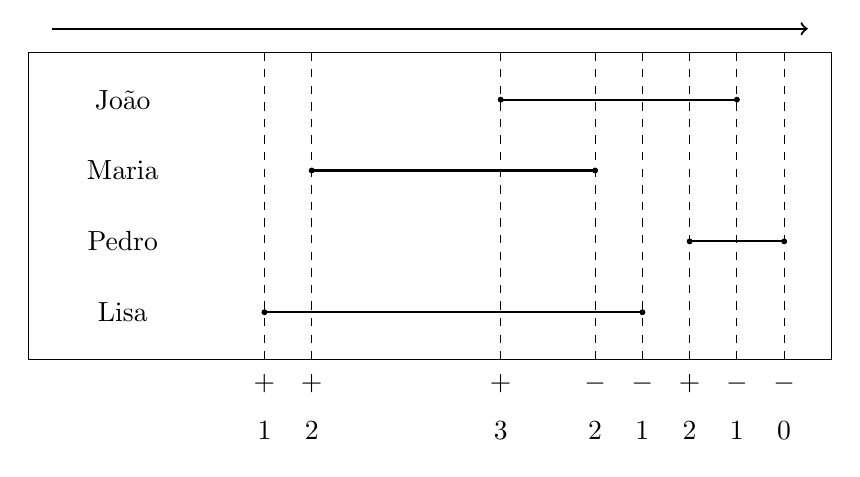
\begin{tikzpicture}[scale=0.6]
\path[draw,thick,->] (0.5,0.5) -- (16.5,0.5);
\draw (0,0) rectangle (17,-6.5);
\path[draw,thick,-] (10,-1) -- (15,-1);
\path[draw,thick,-] (6,-2.5) -- (12,-2.5);
\path[draw,thick,-] (14,-4) -- (16,-4);
\path[draw,thick,-] (5,-5.5) -- (13,-5.5);

\draw[fill] (10,-1) circle [radius=0.05];
\draw[fill] (15,-1) circle [radius=0.05];
\draw[fill] (6,-2.5) circle [radius=0.05];
\draw[fill] (12,-2.5) circle [radius=0.05];
\draw[fill] (14,-4) circle [radius=0.05];
\draw[fill] (16,-4) circle [radius=0.05];
\draw[fill] (5,-5.5) circle [radius=0.05];
\draw[fill] (13,-5.5) circle [radius=0.05];

\node at (2,-1) {João};
\node at (2,-2.5) {Maria};
\node at (2,-4) {Pedro};
\node at (2,-5.5) {Lisa};

\path[draw,dashed] (10,0)--(10,-6.5);
\path[draw,dashed] (15,0)--(15,-6.5);
\path[draw,dashed] (6,0)--(6,-6.5);
\path[draw,dashed] (12,0)--(12,-6.5);
\path[draw,dashed] (14,0)--(14,-6.5);
\path[draw,dashed] (16,0)--(16,-6.5);
\path[draw,dashed] (5,0)--(5,-6.5);
\path[draw,dashed] (13,0)--(13,-6.5);

\node at (10,-7) {$+$};
\node at (15,-7) {$-$};
\node at (6,-7) {$+$};
\node at (12,-7) {$-$};
\node at (14,-7) {$+$};
\node at (16,-7) {$-$};
\node at (5,-7) {$+$};
\node at (13,-7) {$-$};

\node at (10,-8) {$3$};
\node at (15,-8) {$1$};
\node at (6,-8) {$2$};
\node at (12,-8) {$2$};
\node at (14,-8) {$2$};
\node at (16,-8) {$0$};
\node at (5,-8) {$1$};
\node at (13,-8) {$1$};
\end{tikzpicture}
\end{center}
Os símbolos $+$ e $-$ indicam se o
valor do contador aumenta ou diminui,
e o valor do contador é mostrado abaixo.
O valor máximo do contador é 3
entre a chegada de João e a saída de Maria.

O tempo de execução do algoritmo é $O(n \log n)$,
porque ordenar os eventos leva tempo $O(n \log n)$
e o restante do algoritmo leva tempo $O(n)$.

\section{Pontos de interseção}

\index{ponto de interseção}

Dado um conjunto de $n$ segmentos de linha, cada um deles sendo
horizontal ou vertical, considere o problema de
contar o número total de pontos de interseção.
Por exemplo, quando os segmentos de linha são
\begin{center}
\begin{tikzpicture}[scale=0.5]
\path[draw,thick,-] (0,2) -- (5,2);
\path[draw,thick,-] (1,4) -- (6,4);
\path[draw,thick,-] (6,3) -- (10,3);
\path[draw,thick,-] (2,1) -- (2,6);
\path[draw,thick,-] (8,2) -- (8,5);
\end{tikzpicture}
\end{center}
existem três pontos de interseção:
\begin{center}
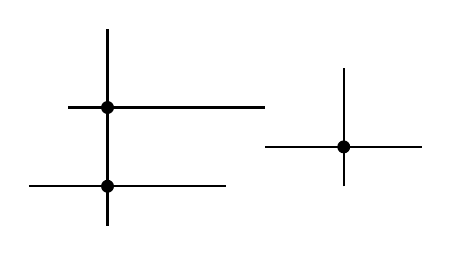
\begin{tikzpicture}[scale=0.5]
\path[draw,thick,-] (0,2) -- (5,2);
\path[draw,thick,-] (1,4) -- (6,4);
\path[draw,thick,-] (6,3) -- (10,3);
\path[draw,thick,-] (2,1) -- (2,6);
\path[draw,thick,-] (8,2) -- (8,5);

\draw[fill] (2,2) circle [radius=0.15];
\draw[fill] (2,4) circle [radius=0.15];
\draw[fill] (8,3) circle [radius=0.15];

\end{tikzpicture}
\end{center}

É fácil resolver o problema em tempo $O(n^2)$,
porque podemos percorrer todos os pares possíveis de segmentos de linha
e verificar se eles se cruzam.
No entanto, podemos resolver o problema de forma mais eficiente
em tempo $O(n \log n)$ usando um algoritmo de linha de varredura
e uma estrutura de dados de consulta de intervalo.

A ideia é processar os pontos finais dos segmentos de linha
da esquerda para a direita e
focar em três tipos de eventos:
\begin{enumerate}[noitemsep]
\item[(1)] segmento horizontal começa
\item[(2)] segmento horizontal termina
\item[(3)] segmento vertical
\end{enumerate}

Os seguintes eventos correspondem ao exemplo:
\begin{center}
\begin{tikzpicture}[scale=0.6]
\path[draw,dashed] (0,2) -- (5,2);
\path[draw,dashed] (1,4) -- (6,4);
\path[draw,dashed] (6,3) -- (10,3);
\path[draw,dashed] (2,1) -- (2,6);
\path[draw,dashed] (8,2) -- (8,5);

\node at (0,2) {$1$};
\node at (5,2) {$2$};
\node at (1,4) {$1$};
\node at (6,4) {$2$};
\node at (6,3) {$1$};
\node at (10,3) {$2$};

\node at (2,3.5) {$3$};
\node at (8,3.5) {$3$};
\end{tikzpicture}
\end{center}

Percorremos os eventos da esquerda para a direita
e usamos uma estrutura de dados que mantém um conjunto de
coordenadas y onde há um segmento horizontal ativo.
No evento 1, adicionamos a coordenada y do segmento
ao conjunto e, no evento 2, removemos a
coordenada y do conjunto.

Os pontos de interseção são calculados no evento 3.
Quando há um segmento vertical entre os pontos
$y_1$ e $y_2$, contamos o número de segmentos horizontais ativos cuja coordenada y está entre
$y_1$ e $y_2$, e adicionamos esse número ao total
de pontos de interseção.

Para armazenar as coordenadas y dos segmentos horizontais,
podemos usar uma árvore de índice binário ou árvore de segmentos,
possivelmente com compactação de índice.
Quando tais estruturas são usadas, o processamento de cada evento
leva $O(\log n)$, então o tempo total de execução
do algoritmo é $O(n \log n)$.

\section{Problema do par mais próximo}

\index{par mais próximo}

Dado um conjunto de $n$ pontos, nosso próximo problema é
encontrar dois pontos cuja distância euclidiana seja mínima.
Por exemplo, se os pontos são
\begin{center}
\begin{tikzpicture}[scale=0.7]
\draw (0,0)--(12,0)--(12,4)--(0,4)--(0,0);

\draw (1,2) circle [radius=0.1];
\draw (3,1) circle [radius=0.1];
\draw (4,3) circle [radius=0.1];
\draw (5.5,1.5) circle [radius=0.1];
\draw (6,2.5) circle [radius=0.1];
\draw (7,1) circle [radius=0.1];
\draw (9,1.5) circle [radius=0.1];
\draw (10,2) circle [radius=0.1];
\draw (1.5,3.5) circle [radius=0.1];
\draw (1.5,1) circle [radius=0.1];
\draw (2.5,3) circle [radius=0.1];
\draw (4.5,1.5) circle [radius=0.1];
\draw (5.25,0.5) circle [radius=0.1];
\draw (6.5,2) circle [radius=0.1];
\end{tikzpicture}
\end{center}
\begin{samepage}
devemos encontrar os seguintes pontos:
\begin{center}
\begin{tikzpicture}[scale=0.7]
\draw (0,0)--(12,0)--(12,4)--(0,4)--(0,0);

\draw (1,2) circle [radius=0.1];
\draw (3,1) circle [radius=0.1];
\draw (4,3) circle [radius=0.1];
\draw (5.5,1.5) circle [radius=0.1];
\draw[fill] (6,2.5) circle [radius=0.1];
\draw (7,1) circle [radius=0.1];
\draw (9,1.5) circle [radius=0.1];
\draw (10,2) circle [radius=0.1];
\draw (1.5,3.5) circle [radius=0.1];
\draw (1.5,1) circle [radius=0.1];
\draw (2.5,3) circle [radius=0.1];
\draw (4.5,1.5) circle [radius=0.1];
\draw (5.25,0.5) circle [radius=0.1];
\draw[fill] (6.5,2) circle [radius=0.1];
\end{tikzpicture}
\end{center}
\end{samepage}

Este é outro exemplo de um problema
que pode ser resolvido em tempo $O(n \log n)$
usando um algoritmo de linha de varredura\footnote{Além desta abordagem,
também existe um
algoritmo de divisão e conquista de tempo $O(n \log n)$ \cite{sha75}
que divide os pontos em dois conjuntos e resolve recursivamente
o problema para ambos os conjuntos.}.
Percorremos os pontos da esquerda para a direita
e mantemos um valor $d$: a distância mínima
entre dois pontos vistos até agora.
Em cada ponto, encontramos o ponto mais próximo à esquerda.
Se a distância for menor que $d$, é a
nova distância mínima e atualizamos
o valor de $d$.

Se o ponto atual é $(x,y)$
e há um ponto à esquerda
a uma distância menor que $d$,
a coordenada x de tal ponto deve
estar entre $[x-d,x]$ e a coordenada y
deve estar entre $[y-d,y+d]$.
Assim, basta considerar apenas os pontos
que estão localizados nesses intervalos,
o que torna o algoritmo eficiente.

Por exemplo, na imagem a seguir, a
região marcada com linhas tracejadas contém
os pontos que podem estar a uma distância de $d$
do ponto ativo:

\begin{center}
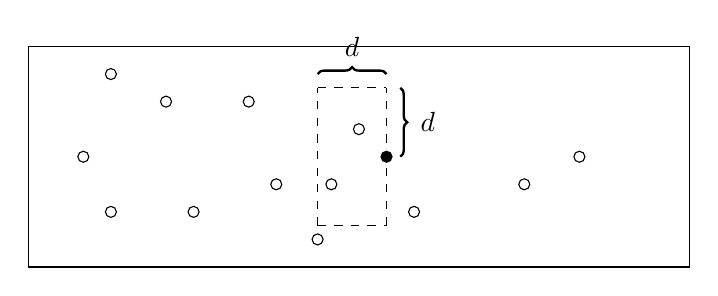
\begin{tikzpicture}[scale=0.7]
\draw (0,0)--(12,0)--(12,4)--(0,4)--(0,0);

\draw (1,2) circle [radius=0.1];
\draw (3,1) circle [radius=0.1];
\draw (4,3) circle [radius=0.1];
\draw (5.5,1.5) circle [radius=0.1];
\draw (6,2.5) circle [radius=0.1];
\draw (7,1) circle [radius=0.1];
\draw (9,1.5) circle [radius=0.1];
\draw (10,2) circle [radius=0.1];
\draw (1.5,3.5) circle [radius=0.1];
\draw (1.5,1) circle [radius=0.1];
\draw (2.5,3) circle [radius=0.1];
\draw (4.5,1.5) circle [radius=0.1];
\draw (5.25,0.5) circle [radius=0.1];
\draw[fill] (6.5,2) circle [radius=0.1];

\draw[dashed] (6.5,0.75)--(6.5,3.25);
\draw[dashed] (5.25,0.75)--(5.25,3.25);
\draw[dashed] (5.25,0.75)--(6.5,0.75);
\draw[dashed] (5.25,3.25)--(6.5,3.25);

\draw [decoration={brace}, decorate, line width=0.3mm] (5.25,3.5) -- (6.5,3.5);
\node at (5.875,4) {$d$};
\draw [decoration={brace}, decorate, line width=0.3mm] (6.75,3.25) -- (6.75,2);
\node at (7.25,2.625) {$d$};
\end{tikzpicture}
\end{center}

A eficiência do algoritmo é baseada no fato
de que a região sempre contém
apenas $O(1)$ pontos.
Podemos percorrer esses pontos em tempo $O(\log n)$
mantendo um conjunto de pontos cuja coordenada x
está entre $[x-d,x]$, em ordem crescente de acordo
com suas coordenadas y.

A complexidade de tempo do algoritmo é $O(n \log n)$,
porque percorremos $n$ pontos e
encontramos para cada ponto o ponto mais próximo à esquerda
em tempo $O(\log n)$.

\section{Problema do fecho convexo}

Um \key{fecho convexo} é o menor polígono convexo
que contém todos os pontos de um determinado conjunto.
Convexidade significa que um segmento de linha entre
quaisquer dois vértices do polígono está completamente
dentro do polígono.

\begin{samepage}
Por exemplo, para os pontos
\begin{center}
\begin{tikzpicture}[scale=0.7]
\draw (0,0) circle [radius=0.1];
\draw (4,-1) circle [radius=0.1];
\draw (7,1) circle [radius=0.1];
\draw (6,3) circle [radius=0.1];
\draw (2,4) circle [radius=0.1];
\draw (0,2) circle [radius=0.1];

\draw (1,1) circle [radius=0.1];
\draw (2,2) circle [radius=0.1];
\draw (3,2) circle [radius=0.1];
\draw (4,0) circle [radius=0.1];
\draw (4,3) circle [radius=0.1];
\draw (5,2) circle [radius=0.1];
\draw (6,1) circle [radius=0.1];
\end{tikzpicture}
\end{center}
\end{samepage}
o fecho convexo é o seguinte:
\begin{center}
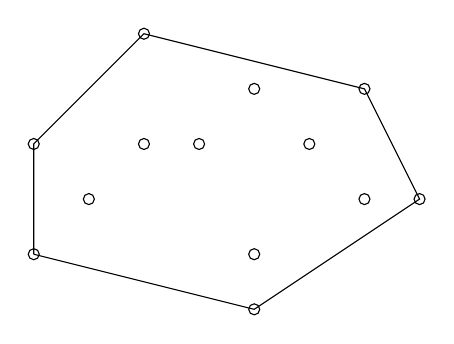
\begin{tikzpicture}[scale=0.7]
\draw (0,0)--(4,-1)--(7,1)--(6,3)--(2,4)--(0,2)--(0,0);

\draw (0,0) circle [radius=0.1];
\draw (4,-1) circle [radius=0.1];
\draw (7,1) circle [radius=0.1];
\draw (6,3) circle [radius=0.1];
\draw (2,4) circle [radius=0.1];
\draw (0,2) circle [radius=0.1];

\draw (1,1) circle [radius=0.1];
\draw (2,2) circle [radius=0.1];
\draw (3,2) circle [radius=0.1];
\draw (4,0) circle [radius=0.1];
\draw (4,3) circle [radius=0.1];
\draw (5,2) circle [radius=0.1];
\draw (6,1) circle [radius=0.1];
\end{tikzpicture}
\end{center}

\index{algoritmo de Andrew}

O \key{algoritmo de Andrew} \cite{and79} fornece
uma maneira fácil de
construir o fecho convexo para um conjunto de pontos
em tempo $O(n \log n)$.
O algoritmo primeiro localiza os pontos mais à esquerda
e mais à direita, e então
constrói o fecho convexo em duas partes:
primeiro o casco superior e depois o casco inferior.
Ambas as partes são semelhantes, então podemos nos concentrar em
construir o casco superior.

Primeiro, ordenamos os pontos primeiramente de acordo
com as coordenadas x e secundariamente de acordo com as coordenadas y.
Depois disso, percorremos os pontos e
adicionamos cada ponto ao casco.
Sempre depois de adicionar um ponto ao casco,
certificamo-nos de que o último segmento de linha
no casco não vire à esquerda.
Enquanto ele virar à esquerda, removemos repetidamente o
penúltimo ponto do casco.

As figuras a seguir mostram como
o algoritmo de Andrew funciona:
\\
\begin{tabular}{ccccccc}
\\
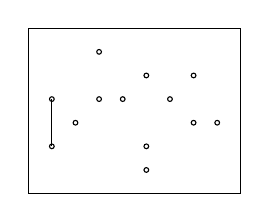
\begin{tikzpicture}[scale=0.3]
\draw (-1,-2)--(8,-2)--(8,5)--(-1,5)--(-1,-2);
\draw (0,0) circle [radius=0.1];
\draw (4,-1) circle [radius=0.1];
\draw (7,1) circle [radius=0.1];
\draw (6,3) circle [radius=0.1];
\draw (2,4) circle [radius=0.1];
\draw (0,2) circle [radius=0.1];

\draw (1,1) circle [radius=0.1];
\draw (2,2) circle [radius=0.1];
\draw (3,2) circle [radius=0.1];
\draw (4,0) circle [radius=0.1];
\draw (4,3) circle [radius=0.1];
\draw (5,2) circle [radius=0.1];
\draw (6,1) circle [radius=0.1];

\draw (0,0)--(0,2);
\end{tikzpicture}
& \hspace{0.1cm} &
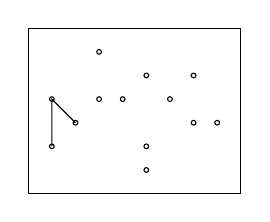
\begin{tikzpicture}[scale=0.3]
\draw (-1,-2)--(8,-2)--(8,5)--(-1,5)--(-1,-2);
\draw (0,0) circle [radius=0.1];
\draw (4,-1) circle [radius=0.1];
\draw (7,1) circle [radius=0.1];
\draw (6,3) circle [radius=0.1];
\draw (2,4) circle [radius=0.1];
\draw (0,2) circle [radius=0.1];

\draw (1,1) circle [radius=0.1];
\draw (2,2) circle [radius=0.1];
\draw (3,2) circle [radius=0.1];
\draw (4,0) circle [radius=0.1];
\draw (4,3) circle [radius=0.1];
\draw (5,2) circle [radius=0.1];
\draw (6,1) circle [radius=0.1];

\draw (0,0)--(0,2)--(1,1);
\end{tikzpicture}
& \hspace{0.1cm} &
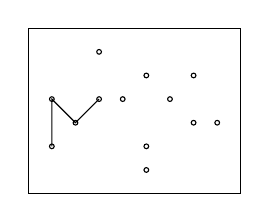
\begin{tikzpicture}[scale=0.3]
\draw (-1,-2)--(8,-2)--(8,5)--(-1,5)--(-1,-2);
\draw (0,0) circle [radius=0.1];
\draw (4,-1) circle [radius=0.1];
\draw (7,1) circle [radius=0.1];
\draw (6,3) circle [radius=0.1];
\draw (2,4) circle [radius=0.1];
\draw (0,2) circle [radius=0.1];

\draw (1,1) circle [radius=0.1];
\draw (2,2) circle [radius=0.1];
\draw (3,2) circle [radius=0.1];
\draw (4,0) circle [radius=0.1];
\draw (4,3) circle [radius=0.1];
\draw (5,2) circle [radius=0.1];
\draw (6,1) circle [radius=0.1];

\draw (0,0)--(0,2)--(1,1)--(2,2);
\end{tikzpicture}
& \hspace{0.1cm} &
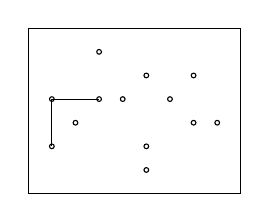
\begin{tikzpicture}[scale=0.3]
\draw (-1,-2)--(8,-2)--(8,5)--(-1,5)--(-1,-2);
\draw (0,0) circle [radius=0.1];
\draw (4,-1) circle [radius=0.1];
\draw (7,1) circle [radius=0.1];
\draw (6,3) circle [radius=0.1];
\draw (2,4) circle [radius=0.1];
\draw (0,2) circle [radius=0.1];

\draw (1,1) circle [radius=0.1];
\draw (2,2) circle [radius=0.1];
\draw (3,2) circle [radius=0.1];
\draw (4,0) circle [radius=0.1];
\draw (4,3) circle [radius=0.1];
\draw (5,2) circle [radius=0.1];
\draw (6,1) circle [radius=0.1];

\draw (0,0)--(0,2)--(2,2);
\end{tikzpicture}
\\
1 & & 2 & & 3 & & 4 \\
\end{tabular}
\\
\begin{tabular}{ccccccc}
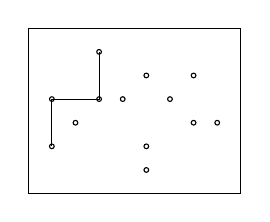
\begin{tikzpicture}[scale=0.3]
\draw (-1,-2)--(8,-2)--(8,5)--(-1,5)--(-1,-2);
\draw (0,0) circle [radius=0.1];
\draw (4,-1) circle [radius=0.1];
\draw (7,1) circle [radius=0.1];
\draw (6,3) circle [radius=0.1];
\draw (2,4) circle [radius=0.1];
\draw (0,2) circle [radius=0.1];

\draw (1,1) circle [radius=0.1];
\draw (2,2) circle [radius=0.1];
\draw (3,2) circle [radius=0.1];
\draw (4,0) circle [radius=0.1];
\draw (4,3) circle [radius=0.1];
\draw (5,2) circle [radius=0.1];
\draw (6,1) circle [radius=0.1];

\draw (0,0)--(0,2)--(2,2)--(2,4);
\end{tikzpicture}
& \hspace{0.1cm} &
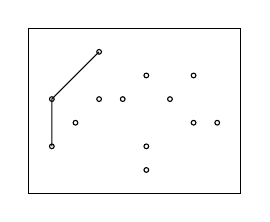
\begin{tikzpicture}[scale=0.3]
\draw (-1,-2)--(8,-2)--(8,5)--(-1,5)--(-1,-2);
\draw (0,0) circle [radius=0.1];
\draw (4,-1) circle [radius=0.1];
\draw (7,1) circle [radius=0.1];
\draw (6,3) circle [radius=0.1];
\draw (2,4) circle [radius=0.1];
\draw (0,2) circle [radius=0.1];

\draw (1,1) circle [radius=0.1];
\draw (2,2) circle [radius=0.1];
\draw (3,2) circle [radius=0.1];
\draw (4,0) circle [radius=0.1];
\draw (4,3) circle [radius=0.1];
\draw (5,2) circle [radius=0.1];
\draw (6,1) circle [radius=0.1];

\draw (0,0)--(0,2)--(2,4);
\end{tikzpicture}
& \hspace{0.1cm} &
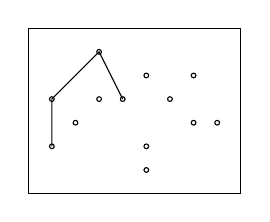
\begin{tikzpicture}[scale=0.3]
\draw (-1,-2)--(8,-2)--(8,5)--(-1,5)--(-1,-2);
\draw (0,0) circle [radius=0.1];
\draw (4,-1) circle [radius=0.1];
\draw (7,1) circle [radius=0.1];
\draw (6,3) circle [radius=0.1];
\draw (2,4) circle [radius=0.1];
\draw (0,2) circle [radius=0.1];

\draw (1,1) circle [radius=0.1];
\draw (2,2) circle [radius=0.1];
\draw (3,2) circle [radius=0.1];
\draw (4,0) circle [radius=0.1];
\draw (4,3) circle [radius=0.1];
\draw (5,2) circle [radius=0.1];
\draw (6,1) circle [radius=0.1];

\draw (0,0)--(0,2)--(2,4)--(3,2);
\end{tikzpicture}
& \hspace{0.1cm} &
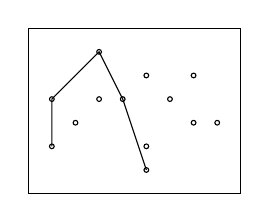
\begin{tikzpicture}[scale=0.3]
\draw (-1,-2)--(8,-2)--(8,5)--(-1,5)--(-1,-2);
\draw (0,0) circle [radius=0.1];
\draw (4,-1) circle [radius=0.1];
\draw (7,1) circle [radius=0.1];
\draw (6,3) circle [radius=0.1];
\draw (2,4) circle [radius=0.1];
\draw (0,2) circle [radius=0.1];

\draw (1,1) circle [radius=0.1];
\draw (2,2) circle [radius=0.1];
\draw (3,2) circle [radius=0.1];
\draw (4,0) circle [radius=0.1];
\draw (4,3) circle [radius=0.1];
\draw (5,2) circle [radius=0.1];
\draw (6,1) circle [radius=0.1];

\draw (0,0)--(0,2)--(2,4)--(3,2)--(4,-1);
\end{tikzpicture}
\\
5 & & 6 & & 7 & & 8 \\
\end{tabular}
\\
\begin{tabular}{ccccccc}
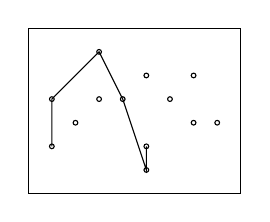
\begin{tikzpicture}[scale=0.3]
\draw (-1,-2)--(8,-2)--(8,5)--(-1,5)--(-1,-2);
\draw (0,0) circle [radius=0.1];
\draw (4,-1) circle [radius=0.1];
\draw (7,1) circle [radius=0.1];
\draw (6,3) circle [radius=0.1];
\draw (2,4) circle [radius=0.1];
\draw (0,2) circle [radius=0.1];

\draw (1,1) circle [radius=0.1];
\draw (2,2) circle [radius=0.1];
\draw (3,2) circle [radius=0.1];
\draw (4,0) circle [radius=0.1];
\draw (4,3) circle [radius=0.1];
\draw (5,2) circle [radius=0.1];
\draw (6,1) circle [radius=0.1];

\draw (0,0)--(0,2)--(2,4)--(3,2)--(4,-1)--(4,0);
\end{tikzpicture}
& \hspace{0.1cm} &
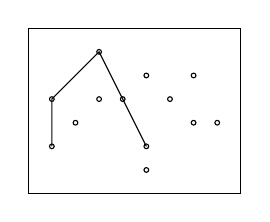
\begin{tikzpicture}[scale=0.3]
\draw (-1,-2)--(8,-2)--(8,5)--(-1,5)--(-1,-2);
\draw (0,0) circle [radius=0.1];
\draw (4,-1) circle [radius=0.1];
\draw (7,1) circle [radius=0.1];
\draw (6,3) circle [radius=0.1];
\draw (2,4) circle [radius=0.1];
\draw (0,2) circle [radius=0.1];

\draw (1,1) circle [radius=0.1];
\draw (2,2) circle [radius=0.1];
\draw (3,2) circle [radius=0.1];
\draw (4,0) circle [radius=0.1];
\draw (4,3) circle [radius=0.1];
\draw (5,2) circle [radius=0.1];
\draw (6,1) circle [radius=0.1];

\draw (0,0)--(0,2)--(2,4)--(3,2)--(4,0);
\end{tikzpicture}
& \hspace{0.1cm} &
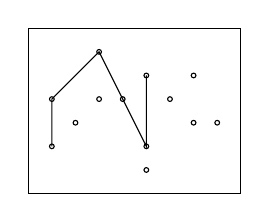
\begin{tikzpicture}[scale=0.3]
\draw (-1,-2)--(8,-2)--(8,5)--(-1,5)--(-1,-2);
\draw (0,0) circle [radius=0.1];
\draw (4,-1) circle [radius=0.1];
\draw (7,1) circle [radius=0.1];
\draw (6,3) circle [radius=0.1];
\draw (2,4) circle [radius=0.1];
\draw (0,2) circle [radius=0.1];

\draw (1,1) circle [radius=0.1];
\draw (2,2) circle [radius=0.1];
\draw (3,2) circle [radius=0.1];
\draw (4,0) circle [radius=0.1];
\draw (4,3) circle [radius=0.1];
\draw (5,2) circle [radius=0.1];
\draw (6,1) circle [radius=0.1];

\draw (0,0)--(0,2)--(2,4)--(3,2)--(4,0)--(4,3);
\end{tikzpicture}
& \hspace{0.1cm} &
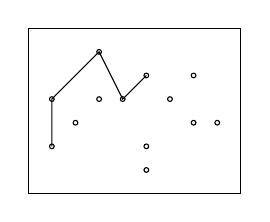
\begin{tikzpicture}[scale=0.3]
\draw (-1,-2)--(8,-2)--(8,5)--(-1,5)--(-1,-2);
\draw (0,0) circle [radius=0.1];
\draw (4,-1) circle [radius=0.1];
\draw (7,1) circle [radius=0.1];
\draw (6,3) circle [radius=0.1];
\draw (2,4) circle [radius=0.1];
\draw (0,2) circle [radius=0.1];

\draw (1,1) circle [radius=0.1];
\draw (2,2) circle [radius=0.1];
\draw (3,2) circle [radius=0.1];
\draw (4,0) circle [radius=0.1];
\draw (4,3) circle [radius=0.1];
\draw (5,2) circle [radius=0.1];
\draw (6,1) circle [radius=0.1];

\draw (0,0)--(0,2)--(2,4)--(3,2)--(4,3);
\end{tikzpicture}
\\
9 & & 10 & & 11 & & 12 \\
\end{tabular}
\\
\begin{tabular}{ccccccc}
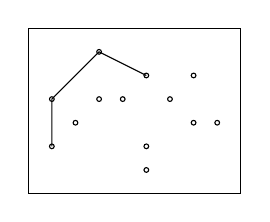
\begin{tikzpicture}[scale=0.3]
\draw (-1,-2)--(8,-2)--(8,5)--(-1,5)--(-1,-2);
\draw (0,0) circle [radius=0.1];
\draw (4,-1) circle [radius=0.1];
\draw (7,1) circle [radius=0.1];
\draw (6,3) circle [radius=0.1];
\draw (2,4) circle [radius=0.1];
\draw (0,2) circle [radius=0.1];

\draw (1,1) circle [radius=0.1];
\draw (2,2) circle [radius=0.1];
\draw (3,2) circle [radius=0.1];
\draw (4,0) circle [radius=0.1];
\draw (4,3) circle [radius=0.1];
\draw (5,2) circle [radius=0.1];
\draw (6,1) circle [radius=0.1];

\draw (0,0)--(0,2)--(2,4)--(4,3);
\end{tikzpicture}
& \hspace{0.1cm} &
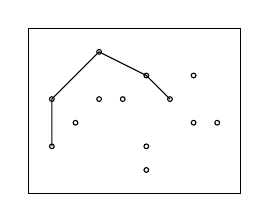
\begin{tikzpicture}[scale=0.3]
\draw (-1,-2)--(8,-2)--(8,5)--(-1,5)--(-1,-2);
\draw (0,0) circle [radius=0.1];
\draw (4,-1) circle [radius=0.1];
\draw (7,1) circle [radius=0.1];
\draw (6,3) circle [radius=0.1];
\draw (2,4) circle [radius=0.1];
\draw (0,2) circle [radius=0.1];

\draw (1,1) circle [radius=0.1];
\draw (2,2) circle [radius=0.1];
\draw (3,2) circle [radius=0.1];
\draw (4,0) circle [radius=0.1];
\draw (4,3) circle [radius=0.1];
\draw (5,2) circle [radius=0.1];
\draw (6,1) circle [radius=0.1];

\draw (0,0)--(0,2)--(2,4)--(4,3)--(5,2);
\end{tikzpicture}
& \hspace{0.1cm} &
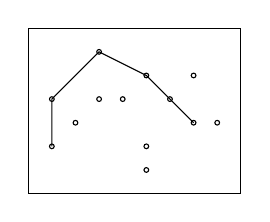
\begin{tikzpicture}[scale=0.3]
\draw (-1,-2)--(8,-2)--(8,5)--(-1,5)--(-1,-2);
\draw (0,0) circle [radius=0.1];
\draw (4,-1) circle [radius=0.1];
\draw (7,1) circle [radius=0.1];
\draw (6,3) circle [radius=0.1];
\draw (2,4) circle [radius=0.1];
\draw (0,2) circle [radius=0.1];

\draw (1,1) circle [radius=0.1];
\draw (2,2) circle [radius=0.1];
\draw (3,2) circle [radius=0.1];
\draw (4,0) circle [radius=0.1];
\draw (4,3) circle [radius=0.1];
\draw (5,2) circle [radius=0.1];
\draw (6,1) circle [radius=0.1];

\draw (0,0)--(0,2)--(2,4)--(4,3)--(5,2)--(6,1);
\end{tikzpicture}
& \hspace{0.1cm} &
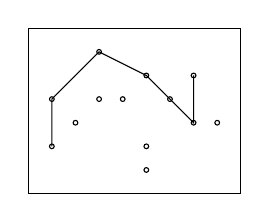
\begin{tikzpicture}[scale=0.3]
\draw (-1,-2)--(8,-2)--(8,5)--(-1,5)--(-1,-2);
\draw (0,0) circle [radius=0.1];
\draw (4,-1) circle [radius=0.1];
\draw (7,1) circle [radius=0.1];
\draw (6,3) circle [radius=0.1];
\draw (2,4) circle [radius=0.1];
\draw (0,2) circle [radius=0.1];

\draw (1,1) circle [radius=0.1];
\draw (2,2) circle [radius=0.1];
\draw (3,2) circle [radius=0.1];
\draw (4,0) circle [radius=0.1];
\draw (4,3) circle [radius=0.1];
\draw (5,2) circle [radius=0.1];
\draw (6,1) circle [radius=0.1];

\draw (0,0)--(0,2)--(2,4)--(4,3)--(5,2)--(6,1)--(6,3);
\end{tikzpicture}
\\
13 & & 14 & & 15 & & 16 \\
\end{tabular}
\\
\begin{tabular}{ccccccc}
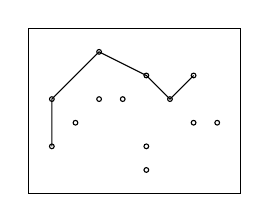
\begin{tikzpicture}[scale=0.3]
\draw (-1,-2)--(8,-2)--(8,5)--(-1,5)--(-1,-2);
\draw (0,0) circle [radius=0.1];
\draw (4,-1) circle [radius=0.1];
\draw (7,1) circle [radius=0.1];
\draw (6,3) circle [radius=0.1];
\draw (2,4) circle [radius=0.1];
\draw (0,2) circle [radius=0.1];

\draw (1,1) circle [radius=0.1];
\draw (2,2) circle [radius=0.1];
\draw (3,2) circle [radius=0.1];
\draw (4,0) circle [radius=0.1];
\draw (4,3) circle [radius=0.1];
\draw (5,2) circle [radius=0.1];
\draw (6,1) circle [radius=0.1];

\draw (0,0)--(0,2)--(2,4)--(4,3)--(5,2)--(6,3);
\end{tikzpicture}
& \hspace{0.1cm} &
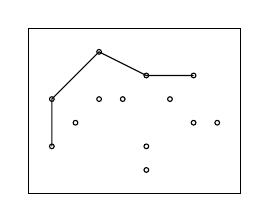
\begin{tikzpicture}[scale=0.3]
\draw (-1,-2)--(8,-2)--(8,5)--(-1,5)--(-1,-2);
\draw (0,0) circle [radius=0.1];
\draw (4,-1) circle [radius=0.1];
\draw (7,1) circle [radius=0.1];
\draw (6,3) circle [radius=0.1];
\draw (2,4) circle [radius=0.1];
\draw (0,2) circle [radius=0.1];

\draw (1,1) circle [radius=0.1];
\draw (2,2) circle [radius=0.1];
\draw (3,2) circle [radius=0.1];
\draw (4,0) circle [radius=0.1];
\draw (4,3) circle [radius=0.1];
\draw (5,2) circle [radius=0.1];
\draw (6,1) circle [radius=0.1];

\draw (0,0)--(0,2)--(2,4)--(4,3)--(6,3);
\end{tikzpicture}
& \hspace{0.1cm} &
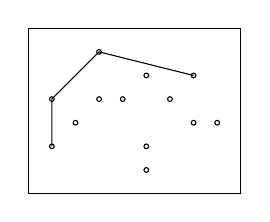
\begin{tikzpicture}[scale=0.3]
\draw (-1,-2)--(8,-2)--(8,5)--(-1,5)--(-1,-2);
\draw (0,0) circle [radius=0.1];
\draw (4,-1) circle [radius=0.1];
\draw (7,1) circle [radius=0.1];
\draw (6,3) circle [radius=0.1];
\draw (2,4) circle [radius=0.1];
\draw (0,2) circle [radius=0.1];

\draw (1,1) circle [radius=0.1];
\draw (2,2) circle [radius=0.1];
\draw (3,2) circle [radius=0.1];
\draw (4,0) circle [radius=0.1];
\draw (4,3) circle [radius=0.1];
\draw (5,2) circle [radius=0.1];
\draw (6,1) circle [radius=0.1];

\draw (0,0)--(0,2)--(2,4)--(6,3);
\end{tikzpicture}
& \hspace{0.1cm} &
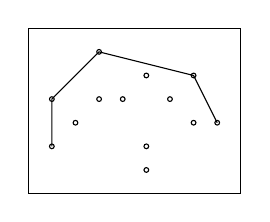
\begin{tikzpicture}[scale=0.3]
\draw (-1,-2)--(8,-2)--(8,5)--(-1,5)--(-1,-2);
\draw (0,0) circle [radius=0.1];
\draw (4,-1) circle [radius=0.1];
\draw (7,1) circle [radius=0.1];
\draw (6,3) circle [radius=0.1];
\draw (2,4) circle [radius=0.1];
\draw (0,2) circle [radius=0.1];

\draw (1,1) circle [radius=0.1];
\draw (2,2) circle [radius=0.1];
\draw (3,2) circle [radius=0.1];
\draw (4,0) circle [radius=0.1];
\draw (4,3) circle [radius=0.1];
\draw (5,2) circle [radius=0.1];
\draw (6,1) circle [radius=0.1];

\draw (0,0)--(0,2)--(2,4)--(6,3)--(7,1);
\end{tikzpicture}
\\
17 & & 18 & & 19 & & 20
\end{tabular}




